\chapter{Descripción del Trabajo}
\label{cap:descripcionTrabajo}

\chapterquote{¡Datos! ¡Datos! ¡Datos! - exclamó con impaciencia - No puedo hacer ladrillos sin arcilla}{El misterio de Copper Beeches\\Arthur Conan Doyle (1892)}

Aquí comienza la descripción del trabajo realizado. Se deben incluir tantos capítulos como sea necesario para describir de la manera más completa posible el trabajo que se ha llevado a cabo. Como muestra la figura, está todo por hacer.

Si te sirve de utilidad,  puedes incluir tablas para mostrar resultados, tal como se ve en la tabla.
\section{Tecnologías utilizadas}\label{s:tech}
Antes de comenzar con el desarrollo del trabajo realizado, en esta sección se introducen las distintas tecnologías que han sido empleadas para la implementación del proyecto. Debe tenerse en cuenta que la totalidad del trabajo ha sido desarrollado usando el lenguaje de programación Python, por lo que las herramientas que se presentan a continuación son compatibles con dicho lenguaje. 

Dado que el estudio gira en torno a los cuerpos de los correos electrónicos, es decir, se centra en el manejo de las cadenas de caracteres, es imprescindible un analizador sintáctico que facilite el análisis del corpus de partida. Para cubrir esta necesidad, se ha elegido spaCy, herramienta que se detalla en la sección \ref{ss:spacy}. Por otro lado, en lo relativo a las tareas relacionadas con el procesamiento de lenguaje natural, también se necesita poder obtener los Information Items dado un texto de entrada. Este problema puede implementarse gracias a la librería textaCy (véase el apartado \ref{ss:textacy}).

En cuanto al desarrollo de la arquitectura transformer, la cual consta de numerosas capas de redes neuronales, como se explicó en la sección \ref{sss:transformer}, será de gran ayuda la librería desarrollada por Google llamada Tensorflow (consúltese el apartado \ref{ss:tf}). Gracias a ella será posible presentar un modelo de aprendizaje automático que aborde todos los problemas de la generación de lenguaje natural.

Por último, se introduce el sistema de almacenamiento con el que se ha trabajado para contar con una gestión eficiente de los datos que se manejan: MongoDB (sección \ref{ss:mongodb}).

\subsection{spaCy}\label{ss:spacy}
Para ser capaces de llegar a conclusiones y estudiar el corpus de correos electrónicos seleccionado (véase la sección \ref{ss:enron}), se debe poder analizar el cuerpo de los mismos. Es decir, se necesita un analizador sintáctico que permita separar los diferentes textos en tokens (o dicho de otro modo, segmentar el texto en palabras, signos de puntuación, etcétera) y obtener diferentes características de ellos (como su categoría gramatical). Para conseguir ese objetivo, se va a utilizar la librería spaCy\footnote{\url{https://spacy.io/}}.

En esta sección se explican las razones por las que se elige spaCy (véase la sección \ref{ssect:spacywhy}) y su utilidad en el proyecto (véase la sección \ref{ssect:spacyut}).

\subsubsection{spaCy frente a otros analizadores sintácticos}\label{ssect:spacywhy}

Se ha elegido spaCy como analizador sintáctico frente a otros por varias razones, apoyadas por investigaciones publicadas como la realizada por \cite{choi2015depends}, y que se explican a continuación.

\begin{figure}[h]
	\centering%
	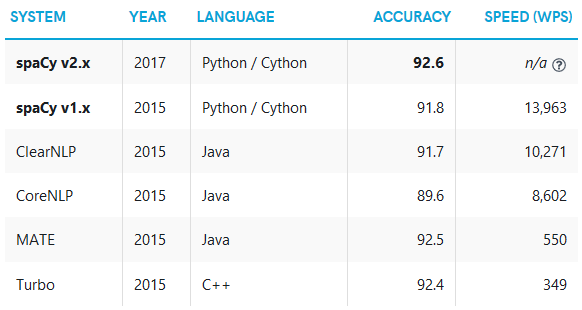
\includegraphics[width = 0.75\textwidth]{Imagenes/Bitmap/spacyeval.png}%
	\caption{Benchmarks de los distintos analizadores sintáctos}%
	Imagen extraída de \url{https://spacy.io/usage/facts-figures#benchmarks}
	\label{fig:spacyeval}
\end{figure}

Una evaluación publicada por \textit{Yahoo! Labs} y la Universidad Emory, como parte de un estudio de las tecnologías de análisis sintáctico actuales \citep{choi2015depends}, observó que ``spaCy es el analizador sintáctico voraz más rápido'' y su precisión está dentro del 1\% de los mejores existentes (como podemos ver en la figura \ref{fig:spacyeval}). Los pocos sistemas que son más precisos son, al menos, 20 veces más lentos. La velocidad es un factor importante cuando se quiere implementar sistemas complejos que se enfrentan a textos largos o a un gran número de documentos (como es el caso de este trabajo, en el que se quieren analizar todos los correos electrónicos posibles).

\begin{figure}[h]
	\centering%
	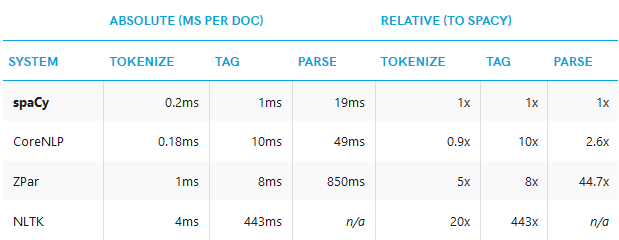
\includegraphics[width = 0.85\textwidth]{Imagenes/Bitmap/spacyspeed.png}%
	\caption{Tiempo de procesamiento por documento de varias librerías de NLP}%
	Imagen extraída de \url{https://spacy.io/usage/facts-figures#benchmarks}
	\label{fig:spacyspeed}
\end{figure}

Los resultados de \cite{choi2015depends} y las discusiones posteriores ayudaron a spaCy a desarrollar una novedosa técnica para mejorar la precisión del sistema, la cual fue publicada en un trabajo conjunto con la Universidad de Macquarie \citep{honnibal2015improved}. Por este motivo, se ha elegido una versión de spaCy que aprovecha esta técnica.

Además, no sólo en general, sino en cada tarea particular (tokenización, etiquetado y análisis sintáctico), spaCy es la más rápida si la comparamos con otras librerías de procesamiento del lenguaje natural. Esto se muestra en la figura \ref{fig:spacyspeed}, donde se puede observar tanto los tiempos absolutos (en milisegundos) como el rendimiento relativo (normalizado a spaCy). Los sistemas que tienen valores más bajos son más rápidos en sus tareas.

\subsubsection{Utilidades de spaCy}\label{ssect:spacyut}
Se puede definir spaCy como una biblioteca de procesamiento de lenguaje natural de Python diseñada específicamente para ser una biblioteca útil para implementar sistemas listos para la producción. Por esta razón, tiene una gran cantidad de utilidades diferentes. Sin embargo, sólo se necesitarán las que realizan el \textit{Tokenizer}.

La clase \textit{Tokenizer} de spaCy se encarga de dividir el mensaje dado en las diferentes palabras que lo constituyen y obtener varias características sobre ellas. Interesan los atributos que se pueden observar en la tabla \ref{tab:attspacy}. Además de su categoría gramatical, da más información (que no nos interesa) en función de su categoría léxica, como su género, número, tiempo verbal o, incluso, el tipo de adverbio.

\begin{table}[h]
	\begin{tabular}{|l|l|p{0.675\linewidth}|}
		\hline
		\textbf{Atributo} & \textbf{Tipo} & \textbf{Explicación}                                                                     \\ \hline
		is\_punct          & bool          & Indica si el token es un signo de puntuación \\ \hline
		is\_right\_punct   & bool          & Indica si el token es un signo de puntuación derecho (como el paréntesis cerrado). \\ \hline
		is\_left\_punct    & bool          & Indica si el token es un signo de puntuación izquierdo\\ \hline
		is\_bracket        & bool          & Indica si el token es un paréntesis\\ \hline
		like\_url          & bool          & Indica si el token es una url \\ \hline
		like\_email        & bool          & Indica si el token es una dirección de correo electrónico\\ \hline
		lema\_             & string        & Forma base del token sin sufijos o inflexiones\\ \hline
		is\_stop           & bool          & Indica si el token es una stop word\\ \hline
		pos\_              & string        & Categoría gramatical\\ \hline
		text & string & Verbatim text content. \\ \hline
		idx & integer & The character offset of the token within the parent document. \\ \hline
	\end{tabular}
	\caption{Atributos de interés de la clase \textit{Tokenizer}}\label{tab:attspacy}
\end{table}


\subsection{textaCy}\label{ss:textacy}

Sobre la librería de spaCy se han desarrollado múltiples soluciones para distintos problemas en el ámbito del procesamiento de lenguaje natural. Uno de estos proyectos es textaCy\footnote{\url{https://spacy.io/universe/project/textacy}}. Se trata de una librería que cuenta con la capacidad de extraer los Information Items (véase la sección \ref{ss:resumen}), definidos como tuplas sujeto-verbo-objeto, de un texto. Basta con añadir la tarea de extracción de los InIts al pipeline de spaCy y, cuando se procese un texto, se obtendrán de forma automática estas tuplas. De esta manera, se puede generar una entrada para los correos electrónicos del corpus (que serían la salida del sistema) con la que entrenar el modelo construido.

\subsection{Tensorflow}\label{ss:tf}
Mientras que spaCy y textaCy son herramientas fundamentales durante el análisis y procesamiento del corpus, la librería de código abierto Tensorflow \citep{abadi2016tensorflow} es la piedra angular del desarrollo de la arquitectura transformer implementada. Posee una amplia cantidad de funcionalidades para trabajar con tensores de manera eficiente, está especializada en los modelos de aprendizaje automático y permite ejecutar Keras utilizando Tensorflow como base, la cual es una librería especialmente diseñada para implementar arquitecturas de deep learning y que facilita la construcción, entrenamiento y evaluación de las mismas.

\subsection{MongoDB}\label{ss:mongodb}
Como se justificará más adelante en la sección \ref{ss:almacen}, se necesita almacenar una gran cantidad de correos electrónicos con el fin de poder trabajar de forma eficiente con ellos. Para esta tarea se ha elegido MongoDB que es un sistema de base de datos NoSQL de código abierto y orientado a documentos.

En lugar de almacenar los datos en tablas, como se hace en las bases de datos relacionales, MongoDB almacena estructuras de datos BSON (una especificación similar a JSON) con un esquema dinámico, lo que facilita y agiliza la integración de datos en determinadas aplicaciones \citep{gyHorodi2015comparative}. Además, no se requieren recursos potentes para trabajar con ella y, gracias a la flexibilidad que ofrece el ser una base de datos NoSQL, se puede realizar fácilmente modificaciones en el modelo conceptual de la base de datos sin tener que preocuparse por los cambios problemáticos entre claves primarias y foráneas entre tablas. Además, cuenta con drivers oficiales para el lenguaje de programación Python con el que se desarrolla la solución.

\section{Análisis de los datos}
El primer paso en todo trabajo de ciencia de datos e inteligencia artificial es el análisis de los datos con los que se cuenta para entrenar y probar el modelo. \textcolor{red}{Completar introducción}

\subsection{Enron corpus}\label{ss:enron}
Para llevar a cabo cualquier trabajo relacionado con la ciencia de datos e inteligencia artificial es necesario contar con un conjunto de datos con el que poder entrenar al modelo desarrollado. Cuando se trata de un estudio relacionado con la generación de lenguaje natural, el conjunto de datos se llama corpus y suele contener ejemplos de documentos reales redactados por humanos similares a los que se desea producir. En concreto, para este trabajo, se ha elegido el corpus conocido como Enron\footnote{\url{http://www-2.cs.cmu.edu/~enron/}}, dado que los correos electrónicos que contiene pertenecieron a la empresa con el mismo nombre. Precisamente se hicieron públicos tras una investigación legal llevada a cabo a esta compañía por parte de la Comisión Federal de Regulación de la Energía\footnote{\url{https://www.ferc.gov/}} de Estados Unidos.

Enron corpus contiene 517.401 correos electrónicos escritos en inglés de 150 usuarios distintos. Además de la ventaja de la gran cantidad de elementos pertenecientes a este dataset, también ha sido elegido por encontrar diversos trabajos sobre este mismo conjunto de e-mails, como el llevado a cabo por \cite{klimt2004introducing}.

Este corpus está organizado en una jerarquía de directorios (uno por cada usuario), en la que dentro de los principales se encuentran las correspondientes carpetas de la cuenta de correo electrónico del usuario en cuestión, como bandeja de entrada, enviados y directorios personalizados. En estas carpetas se encuentran, cada uno en un archivo separado, los distintos correos electrónicos del corpus. Un ejemplo de cómo se presentan los diferentes e-mails viene reflejado en la figura \ref{fig:emailenron}.

\begin{figure}[h]
	\centering%
	\centerline{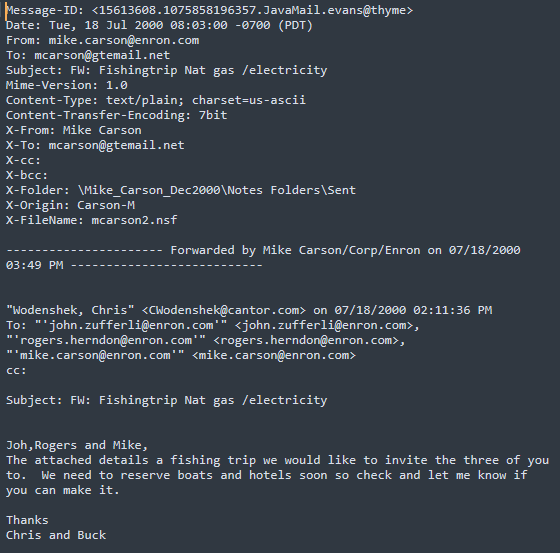
\includegraphics[width = 0.9\textwidth]{Imagenes/Bitmap/email-example.png}}%
	\caption{Ejemplo de un correo electrónico del corpus Enron}%
	\label{fig:emailenron}
\end{figure}

Como puede observarse en la figura \ref{fig:emailenron}, cada uno de los correos electrónicos se encuentra en un archivo distinto estructurado según el formato MIME explicado anteriormente (véase la sección \ref{ss:mime}). Claramente, se pueden diferenciar las distintas cabeceras de este formato con la información correspondiente a cada una de ellas. Después de todas estas cabeceras, se encuentra el cuerpo del mensaje. Por cada uno de los 517.401 correos electrónicos, se encuentra un archivo diferente con esta estructura.

\subsection{Preparación y limpieza de los datos}\label{ss:prep}

El primer problema que aparece ante el conjunto de datos elegidos es el formato en que se presentan cada uno de los correos electrónicos, ya que en cada archivo hay mucha información que generaría ruido y dificultaría el entrenamiento del modelo si no se eliminara (como las cabeceras MIME). Por ese motivo, es necesario preprocesar cada uno de ellos. Asimismo, se conseguiría un dataset apto para el propósito de construir un sistema de generación de lenguaje natural que redacte correos electrónicos.

Para extraer la información relevante de cada uno de ellos, el lenguaje de programación \textit{Python} cuenta con una librería\footnote{\url{https://docs.python.org/3/library/email.parser.html}} capaz de parsear correos electrónicos almacenados en archivos y cadenas de caracteres en formato MIME. Además, una vez procesadas las cadenas, la clase devuelta cuenta con una serie de métodos que facilitan la obtención de la información de las cabeceras y recorrer el árbol de partes MIME (véase la sección \ref{ss:mime} o consúltese el ejemplo de árbol representado en la figura \ref{fig:content-type}). De manera que solo ha sido necesario desarrollar un método que vaya recorriendo la estructura arbórea, comprobando el tipo MIME del nodo, y extrayendo el cuerpo del mensaje cuando lo encuentre.

Una vez se ha resuelto el problema de recuperar el correo electrónico dado el archivo perteneciente al corpus, es posible enfrentarse a otro reto antes del análisis exploratorio de los datos: la limpieza del cuerpo del mensaje para contar con un texto plano de cara al entrenamiento del modelo. Siempre, en todo trabajo en ciencia de datos, se presenta una fase de limpieza de los datos. Este paso resulta ligeramente más complicado cuando se está tratando con cadenas de caracteres. En el caso que ocupa a este trabajo, la limpieza consiste en encontrar patrones externos al cuerpo del mensaje, como la firma o la inclusión del mensaje al que se responde debajo de la respuesta, que no constituyen texto escrito por los usuarios, sino que ha sido incluido por el servidor de correo electrónico. Por ejemplo, en la figura \ref{fig:emailenron}, se muestra un e-mail el cual simplemente está reenviando otro mensaje distinto sin incluir más información. Esto resulta evidente por el comienzo del cuerpo del correo electrónico, que indica el reenvío. Este e-mail no debería incluirse en el entrenamiento de nuestro modelo, porque no añade información nueva y repite un mensaje que ya se tiene en otro archivo (dado que se cuenta con todos los correos del usuario, si el usuario está reenviando un e-mail, significa que es posible encontrar el mensaje original en la bandeja de entrada o alguna de las otras carpetas de su cuenta de correo). Por este motivo, es indispensable limpiar el cuerpo de los todos correos electrónicos del corpus.

Tras analizar concienzudamente el corpus de correos electrónicos se detectan varios patrones que deben abordarse y cambios que tienen que llevarse a cabo en los mensajes. El primero de ellos consiste en que, cuando un usuario contesta a un mensaje, el servidor incluye el mensaje que es respondido debajo de la contestación. En este caso solo interesa la respuesta y no el texto original (pues estará en otro archivo). No obstante, esta casuística no constituye un problema complicado de solventar, ya que se puede distinguir la respuesta del mensaje original porque siempre se incluye una cabecera de texto que no varía. Es decir, basta con encontrar la cabecera como subcadena en el cuerpo y eliminar todo lo que le preceda. La misma solución puede aplicarse al patrón que aparece cuando se envía un correo electrónico modificando una convocatoria de reunión. Resulta que el servidor genera una cabecera para diferenciar la modificación de la convocatoria original.

Ligeramente más complicado respecto a los patrones anteriores, aunque no demasiado, resulta el caso que se muestra en la figura \ref{fig:emailenron}. Se trata del reenvío de un e-mail. Cuando esto ocurre, la cabecera producida por el servidor no se trata de una subcadena fija, sino que incluye como información variable adicional el nombre del usuario que reenvía el correo, así como la fecha y hora en que se produce dicho reenvío. Aunque la solución sea la misma, eliminar lo que preceda a esta cabecera, no basta con buscar una subcadena que no varía, se requiere la utilización de expresiones regulares \citep{thompson1968programming}. Como la gran mayoría de lenguajes de programación, Python cuenta con un módulo para implementar expresiones regulares\footnote{\url{https://docs.python.org/3/library/re.html}} que ha facilitado enormemente esta tarea y ha hecho posible la limpieza de los mensajes con este patrón.

Otro problema que ha sido necesario abordar es el de la firma de los servidores de correo (frases al final de los mensajes como ``Get your FREE download of MSN Explorer''). Al ser siempre iguales, simplemente ha bastado con detectarlos y eliminar dicha subcadena del cuerpo de los mensajes. La dificultad de este tipo de limpieza de texto en realidad reside en detectar estos patrones, ya que, al tratarse de cadenas de caracteres, es complicado detectar incongruencias o errores.

Por último, debido al formato establecido por el protocolo MIME (por lo general depende de la codificación especificada para el mensaje), los servidores de correo electrónico incluyen tabulaciones y saltos de línea con una determinada frecuencia entre las palabras del texto, incluso aunque el usuario no los haya introducido. Dado que el salto de línea o la tabulación no es una información que se considere relevante de cara a la generación de texto de este modelo, se decide transformar estos caracteres en espacios y, a continuación, aplicar las expresiones regulares para detectar las subcadenas en las que se observe más de un espacio en blanco seguido y sustituirlas por uno solo.

Con esto concluye la limpieza de los cuerpos de los mensajes y la fase de preparación de los datos para adaptar los correos electrónicos a un formato adecuado para el sistema de almacenamiento elegido.

\subsection{Procesado y almacenamiento}\label{ss:almacen}

Como se ha explicado en el apartado \ref{ss:enron}, por defecto el corpus se almacena localmente estructurado en una jerarquía de directorios y contando con un archivo por cada correo electrónico. Sin embargo, esta forma de almacenamiento no resulta la más adecuada debido a que imposibilita cualquier método de búsqueda eficiente (sería necesario, en el peor de los casos, abrir todos los archivos para encontrar, por ejemplo, un e-mail en función del identificador del mensaje) y resulta excesivamente lento cuando se pretende procesar todos los mensajes (requiere recorrer la jerarquía como una estructura de datos arbórea entrando en todos los directorios). Por estas razones, la decisión de cambiar el sistema de almacenamiento es acertado para agilizar tanto la carga del corpus como las distintas operaciones que se pueden querer llevar a cabo sobre el mismo.

Como los elementos del conjunto son textos, es decir, datos no estructurados, un almacenamiento clásico en archivos de extensión \textit{.csv} podría provocar problemas como la elección del separador de los distintos campos, habría que utilizar un caracter que no apareciera en ningún cuerpo de mensaje ni en sus otras propiedades (asunto, identificador, destinatario, emisor, etcétera). Por lo tanto, un sistema relacional no parece que sea la mejor opción de almacenamiento para los correos electrónicos. Ante esta situación, se ha elegido el uso del sistema de base de datos NoSQL MongoDB (léase la sección \ref{ss:mongodb}) alojado en la nube\footnote{\url{www.mongodb.com/cloud}}. La decisión de no implantarlo en un repositorio local se sustenta sobre la ventaja que ofrece la nube de disponibilidad desde cualquier dispositivo, lo cual ha sido de gran ayuda en el proceso de desarrollo del trabajo.

Una vez se ha seleccionado la forma de almacenamiento, queda por determinar las colecciones que se van a crear y los campos de los que dispondrán los documentos. Una colección que es indispensable es la que albergará los correos electrónicos, la cual contará con la siguiente estructura:

\begin{python}
{
	# Identificador del documento mongo
	'_id' : ObjectId,
	# Identificador MIME del mensaje
	'Message-ID' : string,
	# Emisor del mensaje
	'From' : string,
	# Destinatario/s del mensaje
	'To' : string,
	# Asunto del mensaje
	'Subject' : string,
	# Cuerpo del mensaje
	'Body' : string,
	# Numero de palabras del cuerpo del mensaje
	'Number_of_Words' : integer,
	# Numero de Information Items del cuerpo del mensaje
	'Number_of_Inits' : integer
}
\end{python}

A excepción de los dos últimos campos, los demás se pueden extraer directamente mediante el uso de la librería específica de Python para mensajes en formato MIME (como se ha explicado en el apartado \ref{ss:prep}). Para obtener los dos últimos, es necesario procesar el cuerpo del mensaje antes de su almacenamiento en la nube. El primero, el número de palabras que contiene el cuerpo del correo electrónico, es posible hallarlo gracias al uso de spaCy (véase la sección \ref{ss:spacy}), librería que no solo tokeniza el texto, sino que nos permite distinguir entre los tokens que son palabras del resto, como, por ejemplo, signos de puntuación.

El último campo del documento que representa a los correos electrónicos, indica el número de Information Items (véase la sección \ref{ss:resumen}) que pueden extraerse del documento siguiendo la implementación llevada a cabo por \cite{genest2010text}. Estos InIts, que se definen como tuplas sujeto-verbo-objeto, se obtienen gracias a la librería textaCy (consúltese el apartado \ref{ss:textacy}), construida a partir de spaCy. De hecho, como se tratará en la sección \textcolor{red}{12345}, las representaciones semánticas abstractas que constituyen los Information Items serán la entrada de nuestro sistema de generación de lenguaje natural, por lo que, para evitar volver a extraerlos (su obtención es una operación computacionalmente costosa), será conveniente almacenarlos como otro documento de MongoDB. Dicha colección poseerá la siguiente estructura:

\begin{python}
	{
		# Identificador del documento mongo
		'_id' : ObjectId,
		# Identificador MIME del mensaje del que se extrajo el InIt
		'Message-ID' : string,
		# Sujeto del InIt
		'Subject' : string,
		# Verbo del InIt
		'Verb' : string,
		# Objeto del InIt
		'Object' : string
	}
\end{python}

Por ejemplo, si en el cuerpo del mensaje aparece la construcción lingüística ``I got change'' (en castellano ``tengo cambios''), se obtendrá el Information Item que se muestra en la figura \ref{fig:initexample}. De esta forma, es posible relacionar fácilmente un correo electrónico con sus InIts y viceversa.

\begin{figure}[h]
	\centering%
	\centerline{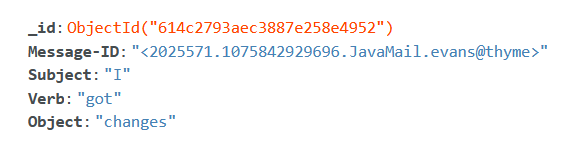
\includegraphics[width = 0.9\textwidth]{Imagenes/Bitmap/initexample.png}}%
	\caption{Ejemplo de documento de un Information Item}%
	\label{fig:initexample}
\end{figure}

Durante el proceso de almacenamiento, también se ha llevado a cabo un primer filtrado de mensajes que no son de utilidad para el propósito que persigue este trabajo y que, por tanto, pueden ser descartados sin guardarlos en MongoDB. Estos son: los correos electrónicos que carecen de cuerpo (puede ser porque originalmente no poseían o porque tras las operaciones de limpieza del mismo que han sido explicadas en la sección \ref{ss:prep}, se produzca esta situación), los e-mails de los que no se extrae ningún Information Item (ya que los InIts serán la entrada de nuestro sistema de generación de lenguaje natural) y los mensajes que son consecuencia de un error en el servidor de mensajería (por ejemplo, al intentar mandar un e-mail con una dirección de destinatario inexistente el servidor de correo siempre manda un mensaje informando de este error). De esta forma, se detectan 35.110 mensajes sin caracteres en el cuerpo, 121.799 correos electrónicos de los que no se extrae ningún Information Item y 7 e-mails consecuencia de errores en el servidor de mensajería, almacenando 360.485 correos electrónicos en la base de datos de MongoDB acompañados de 3.407.099 Information Items.

\subsection{Análisis exploratorio de los datos}\label{ss:eda}
Tras llevar a cabo las tareas de preparación, limpieza de los datos, procesamiento y almacenamiento, con un filtrado a priori, se pueden observar las distribuciones numéricas del corpus desarrollando un análisis exploratorio de los datos. Este estudio preliminar ofrecerá una descripción acerca de los correos electrónicos y sus Information Items.

El primer, y probablemente más sencillo, parámetro que puede analizarse es el número de palabras de cada correo. Para observar cómo se distribuye esta variable en el conjunto de datos, se han calculado las frecuencias requeridas para generar la figura \ref{fig:distpal}. En ella puede deducirse que, a pesar de poseer correos electrónicos con una gigantesca cantidad de palabras, la mayoría de mensajes muestran un número más considerable para tratarse de e-mails.

\begin{figure}[h]
	\centering%
	\centerline{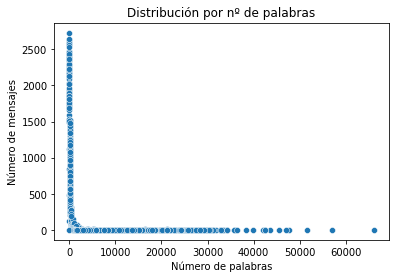
\includegraphics[width = 0.6\textwidth]{Imagenes/Bitmap/dist-palabras.png}}%
	\caption{Distribución del número de palabras en los mensajes}%
	\label{fig:distpal}
\end{figure}
\section{Implementación de una arquitectura realizer}\label{s:realizer}

El planteamiento inicial de este estudio era el de desarrollar una arquitectura realizer que fuera capaz de redactar correos electrónicos de manera automática. Como se explicó detalladamente en la sección \ref{sss:realizer}, el primer problema que surge ante esta propuesta son las estructuras de datos ad hoc generadas en función del dominio del que se quiere producir los textos de lenguaje natural. Esto resulta un inconveniente debido a que, a diferencia de aplicaciones con un dominio definido como pueden ser aquellas cuyo propósito es el de generar informes meteorológicos, la redacción automática de correos electrónicos resulta extremadamente difícil de enmarcar dentro de uno o varios dominios específicos. Además, el corpus que se ha elegido para entrenar el modelo, no se restringe a un tipo de temática de e-mails, sino que pueden encontrarse mensajes que versan sobre una gran variedad de temáticas. Esto complica más la implementación porque, aunque se limitara a un número razonable de asuntos y este hecho no fuera desvelado, el modelo podría ser capaz de aprender el lenguaje específico y las características lingüísticas inherentes a los dominios (por supuesto con mayor dificultad que si se fuera consciente de esta ventaja). Sin embargo, al no contar con esta facilidad, no existen entidades concretas o propiedades comunes más allá de las que posee el lenguaje general.

Si se estudia en detalle la arquitectura realizer, se observa que el mayor problema de restricción de dominio se encuentra en la fase de determinación del contenido. Por supuesto que en el resto de fases también está presente en mayor o menor medida, por ejemplo en la estructuración del documento, pero no posee tanta dependencia como esta primera tarea localizada en el pipeline de las arquitecturas de generación de lenguaje natural. La razón es que resulta sumamente complicado conceptualizar en una estructura de datos concreta, cualquier posible intención que se pueda tener a la hora de transmitir cualquier información. Aún así, la solución traída desde el ámbito del resumen abstractivo de textos, en la que dichas intenciones se materializan en tuplas sujeto-verbo-objeto, solucionaba en gran medida la dificultad del paso de determinación de contenido. Es decir, esta fase se resolvía mediante la generación de Information Items que indican los temas que se desean tratar a lo largo de todo el correo electrónico. De hecho, la gran ventaja de llevar a cabo esta aproximación es que, no solo abordaba el problema de determinación del contenido que, en principio, parecía insalvable, sino que también ofrecía una solución para generar la entrada para el entrenamiento del sistema. Dicho de otro modo, el corpus elegido no proporciona más que los correos electrónicos, que en teoría son la salida final del sistema de generación de lenguaje natural, por lo que no se cuenta con una entrada. Con la solución de las tuplas sujeto-verbo-objeto, es posible conseguir una supuesta entrada desde la que podrían haberse redactado los mensajes. Esto da paso a la utilización de técnicas de aprendizaje supervisado y evita tener que producir una entrada escrita a mano. En resumidas cuentas, con los Information Items ``matábamos dos pájaros de un tiro'': se conseguía un método de generación automática de una entrada para los correos electrónicos ya generados y se solventaba el problema de no ser capaces de concretar el dominio de los e-mails del corpus de cara a diseñar estructuras de datos ad hoc necesarias para implementar la fase de determinación del contenido. Sin embargo, los Information Items introducen un problema sumamente complicado de abordar. Al tratarse de estructuras genéricas que pueden versar sobre cualquier temática, esto impide que puedan usarse técnicas que añadan algún tipo de información adicional en la generación del texto. El origen de este gran escollo es que las fases subsiguientes a la determinación de contenido son altamente dependientes de la salida de esta última. Cuando el dominio es concreto se puede razonar sobre el contenido (con técnicas como las ontologías) o contar con entidades preestablecidas para añadir información extra al texto producido, mientras que al no poder enmarcarse dentro de uno o varios dominios, actualmente no existe la forma de razonar sobre conocimiento general. En consecuencia, el sistema de generación de lenguaje natural se limitaría a recibir las tuplas sujeto-verbo-objeto y construir estructuras lingüísticas que incluyeran única y exclusivamente la información semántica que transmiten los InIts en cuestión. Es decir, simplemente se podrían producir, a lo sumo, tantas oraciones como Information Items se recibiera y la única tarea sería la de generar las escasas estructuras sintácticas que faltaran, así como ajustar algunas categorías morfológicas como el tiempo de los verbos y el género y número de las palabras. Esta técnica de Information Items solo ha sido empleada en los sistemas de resumen automático de textos, precisamente porque impide que en el resto de fases se pueda añadir información adicional más allá de estructuras sintácticas necesarias para la correcta construcción de las oraciones.

Ante este panorama en que las fases subsiguientes a la determinación de contenido poseen una dependencia excesivamente alta cuando se utilizan los Information Items, se descartó la posibilidad de desarrollar este sistema siguiendo el esquema de arquitectura realizer y se optó por generar la aplicación siguiendo el modelo transformer.
\section{Implementación de la arquitectura transformer}\label{s:transformer}

A diferencia de los problemas que se encuentran al tratar de construir una arquitectura realizer para un problema sin dominio específico como es la redacción automática de correos electrónicos, los transformers son capaces de afrontar la generación de lenguaje natural sin la necesidad de enmarcar los textos dentro de un ámbito concreto. De hecho, normalmente se suele acudir a esta arquitectura cuando se pretende hacer frente a problemas en los que podría requerirse un conocimiento general.

Como en el apartado \ref{sss:transformer}, se entró bastante en detalle en la estructura de la arquitectura, cada uno de sus módulos y la filosofía detrás de cada uno de ellos, esta sección se limitará a exponer las vicisitudes específicas del problema que compete a este trabajo, empezando por la entrada de la aplicación.

La entrada del modelo debe ser un conjunto de no más de seis Information Items construidos como tuplas sujeto-verbo-objeto. Sin embargo, esto no coincide del todo con la definición de la entrada del modelo transformer. Para resolverlo, en primer lugar se tomará la lista de todos los InIts y se tokenizarán por separado. La tarea de tokenización se lleva a cabo utilizando un tokenizador preentrenado\footnote{\url{https://www.tensorflow.org/text/api_docs/python/text/BertTokenizer}}.

Con una lista de las tuplas Inits tokenizadas, se concatenan como si constituyeran un solo tensor. Esto podría generar la preocupación de que es necesario antes homogeneizar los tensores asegurándose de que todos los sujetos poseen la misma longitud mediante la técnica de \textit{padding} (todos los tensores se adaptan a la longitud del mayor de ellos rellenando con ceros las últimas dimensiones), y lo mismo con los verbos y objetos. No obstante, además de ser una operación computacionalmente costosa, no es necesario para el correcto funcionamiento de nuestro modelo. El motivo por el que se pueden concatenar los InIts (sobra decir que siempre todos ellos deben seguir el orden sujeto-verbo-objeto, ya que esto sí podría dificultar el entrenamiento y confundir al modelo) y luego hacer padding es que, como se explicó en la sección \ref{sss:transformer}, existen tokens especiales de inicio y fin. Estos se añaden a cada sujeto, verbo y objeto por separado, quedando así todos los elementos claramente delimitados. Es decir, la red neuronal aprenderá a distinguir dónde acaba un elemento de la tupla InIt y dónde comienza el siguiente sin necesidad de incluir ceros entre ellos. Este hecho, no solo ahorra tiempo computacionalmente hablando, sino que también ahorra en memoria, pues los vectores tokenizados de InIts son notablemente más pequeños, y, al reducir el tamaño de los vectores de Information Items, disminuye la entrada de la red y, por ende, el número de parámetros a entrenar.

Tras construir la tokenización de los Information Items, se tokeniza, con el mismo tokenizador preentrenado, el correo electrónico ``resultante''. Así ya se cuenta con la entrada, el tensor concatenado de InIts, y la salida de la red, el tensor del cuerpo del mensaje tokenizado. De esta manera, se está en disposición de entrenar el modelo y evaluar los resultados obtenidos.